\chapter{Objetivos del proyecto}

%\newpage
%Objetivos, alcance, planificación temporal, herramientas, 
%gestión de riesgos, evaluación económica

\section{Objetivos}
Los objetivos del proyecto consisten en crear un software que extienda la funcionalidad actual del sistema INTRASIM desarrollado 
por la universidad de Navarra y del grupo de investigación GALAN perteneciente a la UPV/EHU.

Es un software que permite gráficamente visualizar las observaciones \footnote{Aquí va una explicación de lo que es una observación} del sistema.
 El objetivo principal es brindar al experto una herramienta para poder señalar gráficamente en que momento de esa observación sucede el hecho concreto que estaban buscando.

La herramienta permite visualizar los datos en bruto tanto en modo v\'{i}deo (si esta disponible), como en modo gr\'{a}fico, con polilineas, histogramas etc. Tales gráficos permiten la selección de rangos.

\section{Alcance}
Aquí va el alcance del proyecto.

\section{Planificaci\'{o}n temporal}
En vez de seguir una planificación clásica, como puede ser COCOMO \footnote{\url{https://en.wikipedia.org/wiki/COCOMO}} o Waterfall \footnote{\url{https://en.wikipedia.org/wiki/Waterfall_model}} he decidido utilizar las metodologías agiles de desarrollo, concretamente Scrum y Kanban

\subsection{Scrum}
Scrum es una serie de herramientas (framework) para la gestión y desarrollo de software basado en un proceso iterativo e incremental. \emph{cita a la wikipedia}

\begin{figure}[h]
    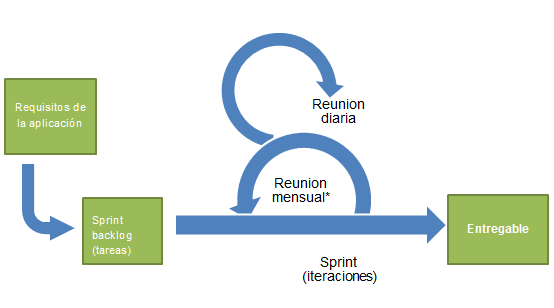
\includegraphics[width=0.7\linewidth]{./Figures/Scrumm}
    \caption[Proceso iterativo Scrum]{En este gráfico podemos ver el método de trabajo según Scrum, en el cual se observa lo importante que son los entregables}
    \label{fig:Scrum}
\end{figure}

%\newpage
Scrum, de manera resumida consiste en lo siguiente:
\begin{enumerate}
    \item Hablar con el cliente para ver si hay nuevos requisitos.
    \item Crear backlog, es decir, las tareas de ese sprint.
    \item Programar los requisitos especificados en el sprint.
    \item Reunión de retrospectiva para ver que ha ido mal y mejorarlo.
    \item Enviar entregable al cliente.
    \item Repetir.
\end{enumerate}

Es fundamental entre sprint y sprint que el valor del producto haya aumentado. Es decir, lo importante es el producto, no como vamos nosotros en el propio proyecto. Podríamos haber avanzado mucho en el diseño del software, pero si eso es algo que el cliente no puede ver estaremos fallando en nuestra agilidad.

Por otro lado, si cometemos algún error será muy sencillo corregir el error ya que si los sprints son de dos semanas por ejemplo, no habremos perdido apenas tiempo. Y además para el cliente los entregables serán predecibles en el tiempo.

Scrum es también muy importante, y se posiciona como una alternativa muy potente frente a COCOMO o waterfall, es porque en la creación de software hay un componente de incertidumbre muy grande. No sabemos como, ni cuando pueden cambiar los requisitos de un software. Por ello toman importancia los sprints de nuevo. 

En los modelos antiguos, si ya habíamos terminado la fase de análisis y diseño, y se requería una nueva funcionalidad es necesario paralizar el desarrollo del software y volver a analizar y diseñar. En cambio, con Scrum es posible integrar ese cambio en el siguiente sprint.

\subsection{Kanban}
Kanban es un método de organización del conocimiento del trabajo que se está realizando con un gran énfasis en el la entrega justo a tiempo \footnote{JIT Delivery: Just-In-Time Delivery} sin sobrecargar al equipo \emph{Cita a la wikipedia}

Kanban se centra mucho en que lo importante no es empezar muchas cosas, si no que acabemos aquello que empezamos. Sirve sobre todo para ver de una manera visual:
\begin{itemize}
    \item Qué tenemos pendiente
    \item Qué estamos haciendo ahora mismo
    \item Qué hemos terminado.
\end{itemize}

El método Kanban es algo muy extenso, pero yo simplemente he aplicado el tablero Kanban mezclado con Scrum. Cada dos semanas, me creo una lista de tareas que debo completar (Backlog) y lo coloco en la columna de "Tareas pendientes", ordenadas por prioridad. Después, coloco en la lista de "En progreso" como máximo dos tareas. Y no empiezo ninguna otra hasta que esas dos hayan sido pasadas a la columna de "Tareas finalizadas".

\subsection{Mi planificaci\'{o}n}
Cada sprint tiene una duraci\'{o}n de un mes, empezando desde Septiembre del 2013.
\subsubsection{Sprint 1}
Este sprint era el comienzo del proyecto, establecer prioridades, documentarse etc. Lo que ha compuesto este sprint ha sido:

\begin{itemize}
    \item Crear y configurar el repositorio Git y los clientes en los dos ordenadores.
    \item Leer la documentaci\'{o}n existente y obtener el c\'{o}digo fuente original.
    \item Iniciar dise\~{n}os gr\'{a}ficos preliminares en papel para elegir las librer\'{i}as necesarias.
    \item Buscar y documentarse sobre las librer\'{i}as que cumplan los requisitos del punto anterior. 
\end{itemize} 

\subsubsection{Sprint 2}
Una vez configurado y elegidas las librer\'{a}s necesarias lo siguiente que se hizo fue:

\begin{itemize}
    \item Reunirse con Mikel para realizar una captura de requisitos.
    \item Dise\~{n}ar unos prototipos funcionales.
    \item Documentar lo que se hab\'{i}a realizado hasta el momento, es decir, el tipo de planificaci\'{o}n que se hab\'{i}a elegido,
    tecnolog\'{i}as que se iban a usar etc.
\end{itemize}

\subsubsection{Sprint 3}
El siguiente paso consiste en poder cargar v\'{i}deos, tantos como se quieran, desde el sistema de archivos.

\begin{itemize}
    \item Crear el control de cargar v\'{i}deos (contenedor de v\'{i}deos). El contenedor debe permitir:
    \begin{itemize}
        \item Cargar distintos v\'{i}deos desde el sistema de archivos.
        \item Cada v\'{i}deo debe disponer de sus controles individuales. Play, pausa, stop y avanzar de tantos segundos en tantos segundos, y que sea
        configurable por el usuario, mediante un archivo de configuraci\'{o}n.
        \item El contenedor de v\'{i}deos debe tener de unos controles generales que pause, y que los reproduzca de manera simultanea
        para mantener la sincronizaci\'{o}n.
        \item Debe permitir establecer para cada v\'{i}deo el momento de inicio del v\'{i}deo manualmente para mantener la sincronizaci\'{o}n.
    \end{itemize}
\end{itemize}

\subsubsection{Sprint 4}
Despu\'{e}s de terminar la visualizaci\'{o}n de v\'{i}deos, lo siguiente en la lista de tareas es crear un visualizador de datos.

\begin{itemize}
    \item Crear el contenedor que nos permita visualizar datos. El control debe permitir:
    \begin{itemize}
        \item Visualizar datos continuos y discretos.
        \item Seleccionar un rango en la gr\'{a}fica, estableciendo un inicio y un fin para un paso.
        \item Que muestre el progreso, y que este sincronizado con el v\'{i}deo.
        \item Guardar el inicio y fin del paso en la base de datos.
        
    \end{itemize}
\end{itemize}

\subsubsection{Sprint 5}
Ya tenemos todo preparado para funcionar, ahora hay que poder guardar datos.

\begin{itemize}
    \item Elegir una Base de Datos.
    \item Configurar los usuarios y permisos de la base de datos.
    \item Crear el diagrama Entidad-Relaci\'{o}n que representara el modo de guardado de datos.
    \item A\~{n}adir al c\'{o}digo existente las llamadas necesarias a la base de datos.
    \item Permitir cambiar la ubicaci\'{o}n de la base de datos mediante un archivo de configuraci\'{o}n.
\end{itemize}

\subsubsection{Sprint 6}
En este momento ya tenemos una aplicaci\'{o}n completamente funcional pero con datos de prueba. Hay que poder cargar datos de los XML.

\begin{itemize}
    \item Crear la clase que lea los XML.
    \item Hablar con Mikel para saber como est\'{a}n guardadas las observaciones.
    \item Utilizando los datos del XML cargar la aplicaci\'{o}n con esos datos.
\end{itemize}

\subsubsection{Observaciones}
N\'{o}tese que hay 6 sprints y desde septiembre hasta junio hay 10 meses. Por lo que se entiende que el resto de tiempo es para:
\begin{enumerate}
    \item Poder realizar las tareas de clase.
    \item Amortiguar el impacto de los retrasos que puedan darse.
\end{enumerate}

\section{Herramientas}
El proyecto, al no ser enteramente mío, no he tenido una libertad total para la elección de herramientas. 

Las herramientas que he utilizado para llevar a cabo este proyecto han sido:
\begin{itemize}
    \item 
    \textbf{Visual Studio}
    
    Para el desarrollo propiamente dicho del proyecto he usado Visual Studio 2013 Ultimate, proporcionado de manera gratuita gracias al acuerdo que mantiene la UPV/EHU con Microsoft.
    
    \item 
    \textbf{TeXstudio y \LaTeX}
    
    Dos herramientas gratuitas y de código abierto para generar documentos.
    
    \item
    \textbf{Git y GitHub}
    
    Fundamental en los proyectos que se basen en metodologías ágiles. Git es un software de gestión de control de versiones distribuido, esto es, que cada desarrollador dispone de una copia completa del repositorio, desarrollado por Linus Torvalds y Junio Hamano en 2005 y similar a SVN.
    
    \item
    \textbf{WPF Toolkit}
    
    Es un a\~{n}adido a la librer\'{i}a WPF est\'{a}ndar que a\~{n}ade una serie de caracte\'{i}sticas que no dispone la configuraci\'{o}n est\'{a}ndar.
    Entre otras cosas a\~{n}ade la posibilidad de manejar gr\'{a}ficos.
    
\end{itemize}

\section{Gesti\'{o}n de riesgos}
Dadas las fechas de entrega impuestas por mi mismo para la finalizaci\'{o}n del Trabajo de Fin de Grado, es un hecho que
aparecerán riesgos que pueden poner en peligro el proyecto. Es por ello que se necesita tener en cuenta las probabilidades de los sucesos que 
pueden ocurrir y que puedan retrasar el trabajo de forma notable. Una vez
listados, se puede proceder a crear un plan de prevención para evitarlos. Y en caso de que la prevención no
funcionara, un plan de contingencia que pueda amortiguar las consecuencias de ese riesgo. A continuación
se listan de forma detallada los riesgos que pueden aparecer durante el transcurso del proyecto.

\subsection{Planificaci\'{o}n}

\subsubsection{Mala concepci\'{o}n del proyecto}

\begin{table}[ht]
    \begin{center}
       \rowcolors{1}{lightgray}{} %\rowcolors{<starting row index>}{<odd row color>}{<even row color>}
       \begin{tabular}{l p{8cm}}
           Descripci\'{o}n                 & Por decisiones erróneas, como puede ser elegir utilizar una
           base de datos, puede que el trabajo deba ser reconstruido desde el principio. \\
           Prevenci\'{o}n                  & Una buena planificación y conocimiento exacto de lo que quiere y necesita el cliente. \\ 
           Plan de contingencia            & Un programa flexible a cambios \\
           Probabilidad                    & Improbable \\
           Impacto                         & Muy alto\\
        \end{tabular}
    \end{center}
    
\end{table}

\subsubsection{Error en la planificaci\'{o}n temporal}

\begin{table}[h]
    \begin{center}
        \rowcolors{1}{lightgray}{} %\rowcolors{<starting row index>}{<odd row color>}{<even row color>}
        \begin{tabular}{l p{8cm}}
            Descripci\'{o}n                 & Por una mala compresión y falta de experiencia el cálculo
            de tiempo estimado de una de las tareas es erróneo y hay que reajustar todo el proyecto. \\
            Prevenci\'{o}n                  & Realizar la estimación lo mejor posible y tener una buena
            comunicación con el cliente para no tener fallos de comprensión. \\ 
            Plan de contingencia            & Margen de error en los tiempos \\
            Probabilidad                    & Muy probable \\
            Impacto                         & Medio\\
        \end{tabular}
    \end{center}
    
\end{table}

\subsection{Organizaci\'{o}n y gesti\'{o}n}

\subsubsection{Incompatibilidad de versiones}

\begin{table}[h]
    \begin{center}
        \rowcolors{1}{lightgray}{} %\rowcolors{<starting row index>}{<odd row color>}{<even row color>}
        \begin{tabular}{l p{8cm}}
            Descripci\'{o}n                 & Al utilizar dos ordenadores, una workstation y un port\'{a}til puede que no disponga de las mismas
            versiones del software o que no se satisfagan todas las dependencias. \\
            Prevenci\'{o}n                  & Asegurarme de disponer el mismo software con las mismas versiones. \\ 
            Plan de contingencia        & Resolver manualmente las dependencias. \\
            Probabilidad                & Probable \\
            Impacto                     & Bajo\\
        \end{tabular}
    \end{center}
    
\end{table}

\section{Viabilidad}
El presente proyecto se ha realizado en colaboraci\'{o}n del grupo GALAN de la UPV/EHU. Concretamente ha sido un proyecto propuesto por ellos
y se entiende que es viable.

\section{Planificaci\'{o}n econ\'{o}mica}
Como el proyecto es en colaboraci\'{o}n de un grupo de investigaci\'{o}n de la UPV/EHU no es necesario estimar los costes ya que
el proyecto se esta realizando bajo el amparo de tal grupo, y se est\'{a} realizando por el bien de la ciencia y del progreso.

%Nuestra empresa la forman:
%\begin{itemize}
%    \item
%    \textbf{Ángel Agudo}: CEO \footnote{Chief Executive Officer: Director ejecutivo} de la empresa.
%    \item
%    \textbf{Asun Santos}: Directora de calidad y administración.
%    \item
%    \textbf{Elena Agudo}: Directora de arte.
%    \item
%    \textbf{Rubén Agudo}: CTO \footnote{Chief Technical Officer: Director de tecnología} y responsable de I+D. 
%\end{itemize}
%Cómo es una epoca complicada por la crisis, tanto Ángel como Asun se han visto en la necesidad de pluriemplearse como administrativos de Osakidetza. 

%Su empleo en Osakidetza reportan a la empresa familiar una cantidad neta de 5000€ mensuales. Nuestro único proyecto de software es este proyecto de fin de %carrera por lo que todos los ingresos provienen de sus otros empleos.

%Como somos una empresa muy concienciada con la investigación y el desarrollo hemos decidido que el proyecto sea gratis y de código abierto, licenciado bajo GPLv3.

%Por lo tanto el coste de venta de nuestro coste sera 0€

%\subsection{Amortizaci\'{o}n de material}
%\subsubsection{Oficina}
%La oficina que utilizamos es el domicilio familiar y no hay que pagar alquiler ya que es de nuestra propiedad. Por lo que el gasto de alquiler/hipoteca es 0€
%\subsubsection{Material inform\'{a}tico}
%El material informático que se ha usado ha sido un portátil Acer TravelMate 5742G comprado en 
%Diciembre de 2010 y usado intensivamente durante estos 4 años. 
%El portátil estaba pensado para ser amortizado en 4 años. \emph{As\'{i} que por aqui habra que hacer algun calculo tonto}

%\subsection{Otros gastos}

%\begin{tabular}{l*{1}{c}r}
%    Concepto                   & Gastos en € / mes & \\
%    \hline
%    Luz                        & 60 & \\
%    Agua                       & 50 & \\
%    Internet + Teléfono        & 60 & \\
%    Gas                        & 70 & \\
%    Seguro                     & 45 & \\
%    IBI                        & 40 & \\
%    \hline
%    Total Mes                  & 325 & \\
%    Total A\~{n}o              & 3900 &\\
%\end{tabular}


%\subsection{Salarios}
%De los 5000€ que se ingresan mensualmente se reparten de la siguiente manera:
%\newline
%\newline
%\begin{tabular}{l*{1}{c}r}
%    Miembro de la empresa     & Salario en € & \\
%    \hline
%    \'{A}ngel Agudo               & 1000 & \\
%    Asun Santos               & 1000 & \\
%    Elena Agudo               & 80 & \\
%    Rubén Agudo               & 80 & \\
%    \hline
%    Remanente Empresa         & 2840 & \\
%\end{tabular}

